\documentclass[xcolor=dvipsnames]{beamer}
\usepackage{xltxtra}
\usepackage[english]{babel}

\xdefinecolor{thecolor}{rgb}{0.5,0.0,0.5}

\mode<presentation>
{
	\usetheme{Rochester}
	\beamertemplatenavigationsymbolsempty
	\usecolortheme[named=thecolor]{structure}
	\setbeamercovered{transparent}
}

\title{SDCC}
\subtitle{Small Device C Compiler}
\date{2025-04-11}

\author{Philipp Klaus Krause}

\subject{Small Device C Compiler, SDCC, C, STM8}

\begin{document}

\begin{frame}
	\titlepage
\end{frame}

\begin{frame}
	\frametitle{What is SDCC?}
	\begin{itemize}
		\item Standard C compiler: ISO C90, ISO C99, ISO C11, ISO C23, ISO C2Y
		\item Freestanding implementation or part of a hosted implementation
		\item Supporting tools (assembler, linker, simulator, ...)
		\item Works on many host systems
		\item Targets various 8-bit architectures, has some unusual optimizations that make sense for these targets
		\item Latest release: 4.5.0 (2025-01-28)
		\item User base: embedded developers and retrocomputing/-gaming enthusiasts
		\item Also used in downstream projects (z88dk, gbdk, devkitSMS)
	\end{itemize}
\end{frame}

\begin{frame}
	\frametitle{Ports}
	\begin{itemize}
		\item MCS-51, DS390, STM8, f8, HC08, S08, PDK13, PDK14, PDK15 (PIC14, PIC16)
		\item MOS 6502, WDC 65C02
		\item Z80, Z80N, Z180, eZ80, TLCS-90, SM83, Rabbits, R800
	\end{itemize}
\end{frame}

\begin{frame}
	\frametitle{Optimal Register Allocation in Polynomial Time}
	\begin{itemize}
		\item Register allocator based on graph-structure theory
		\item Optimal register allocation in polynomial time
		\item Flexible through use of cost function
		\item Provides substantial improvements in code quality
		\item Slow compilation for targets with many registers
		\item Compilation speed / code quality trade-off: --max-allocs-per-node
	\end{itemize}
\end{frame}

\begin{frame}
	\frametitle{Bytewise Register Allocation and Spilling}
	\begin{itemize}
		\item Decide on the storage of variables bytewise
		\item Decide for each individual byte in a variable whether to store it in memory or a register
		\item Consider any byte of any register as a possible storage location
	\end{itemize}
\end{frame}

\begin{frame}
	\frametitle{SDCC vs.\ non-free compilers: STM8 Benchmark scores}
	\centerline{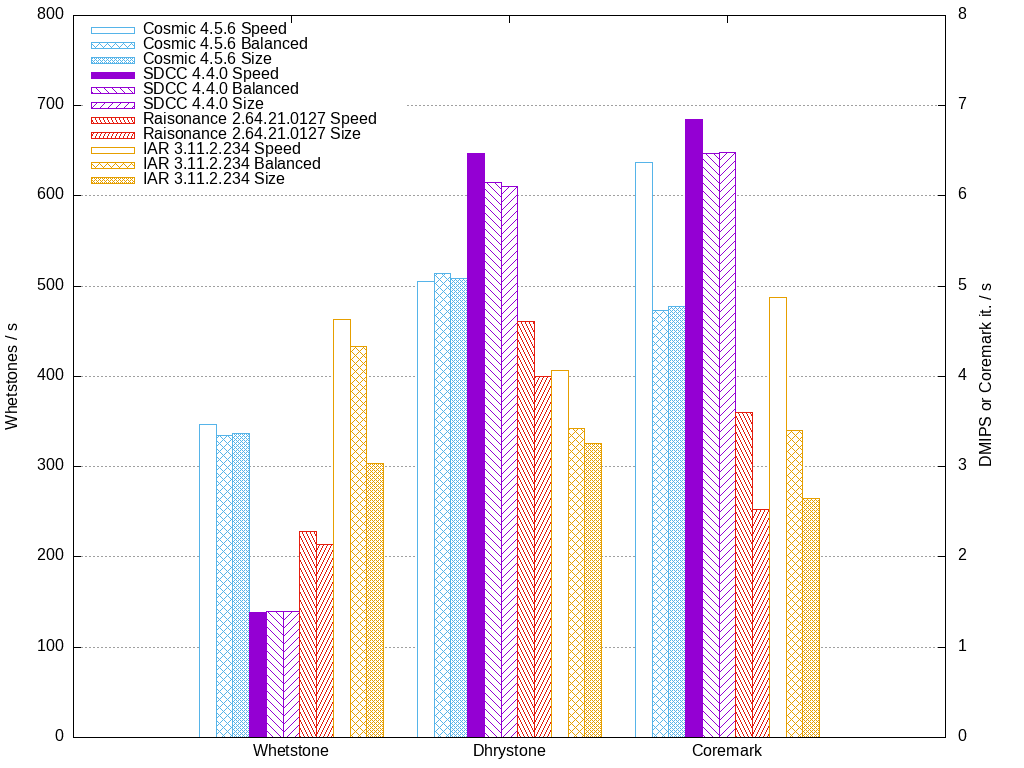
\includegraphics[scale=0.38]{scores-2024.png}}
\end{frame}

\begin{frame}
	\frametitle{SDCC vs.\ non-free compilers: STM8 Code size}
	\centerline{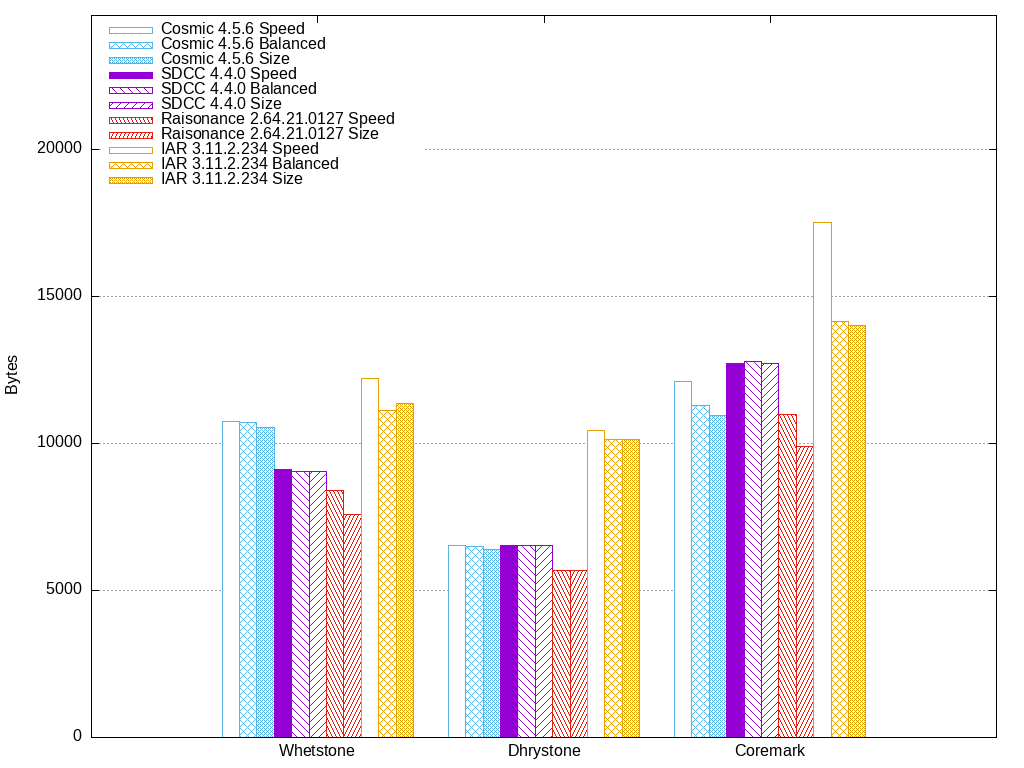
\includegraphics[scale=0.38]{sizes-2024.png}}
\end{frame}

\begin{frame}
	\frametitle{Regression testing}
	\begin{itemize}
		\item Regression testing of nightly snapshots
		\item $\approx 32000$ tests (thrice as many as 2020) compiled and executed on simulators
		\item Tests mostly from fixed bugs and from GCC
		\item Targets architectures: MCS-51, DS390, Z80, Z180, eZ80, Rabbit 2000, Rabbit 2000A, Rabbit 3000A, SM83, TLCS-90, HC08, S08, STM8, PDK14, PDK15. 
		\item Host OS: GNU/Linux, macOS, ``Windows'' (cross-compiled on GNU/Linux, tested via wine)
		\item Host architectures: x86, amd64, ppc64, aarch64
	\end{itemize}
\end{frame}

\begin{frame}
	\frametitle{Challenges}
	Many target architectures of SDCC have been discontinued. How can SDCC stay relevant outside of the retrocomputing niche?
	\begin{itemize}
		\item STM8 - SDCC is doing well, and ST put many STM8 devices back to active
		\item MCS-51 - SDCC port needs major work to be competitive vs. Keil
		\item PDK - Not an easy target for a C compiler
		\item ALP - Don't know much about current state
		\item S08 - SDCC port needs some work, hard to get into dev community
		\item f8
		\item eZ80 - hard to get into dev community
		\item TLCS-870/C1 - no SDCC port yet, hard to get into dev community
	\end{itemize}
\end{frame}

\end{document}

